\section{Utilisation de la plateforme}
  Pour lancer l'application, il suffit d'avoir lancé le serveur Tomcat puis d'ouvrir dans navigateur web la bonne URL. Par exemple : http://localhost:8080/Plateforme/accueil.jsp.
    
  \subsection{Accueil}
  Le joueur arrive donc sur une page d'accueil sur laquelle deux options s'offrent à lui : s'inscrire ou se connecter. Prenons le cas d'un nouveau joueur et inscrivons-le.
  \begin{figure}[H]
    \center
    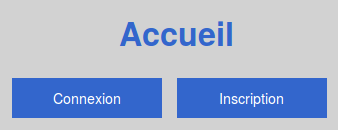
\includegraphics[scale=0.5]{../graph/1-accueil.png} 
  \end{figure}
    
    \subsubsection{Inscription}
    Après avoir cliqué sur le bouton \textbf{Inscription}, la formulaire suivant s'affiche :
    \begin{figure}[H]
      \center 
      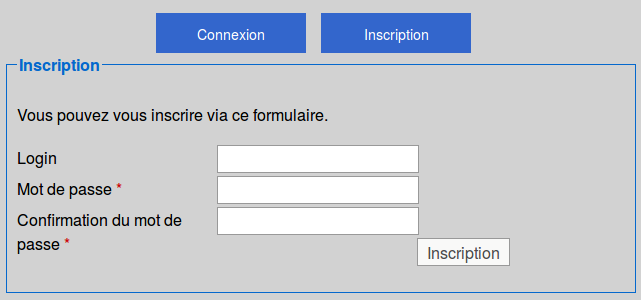
\includegraphics[scale=0.5]{../graph/2-inscription.png} 
    \end{figure}    
    Le joueur saisi alors son login et son mot de passe deux fois, sachant que s'il ne met pas deux fois le même mot de passe, ou s'il tente d'utiliser un login déjà existant un message d'erreur sera affiché (en rouge), sinon un message vert indiquera que l'inscription a bien été effectuée.
    \begin{figure}[H]
      \center 
      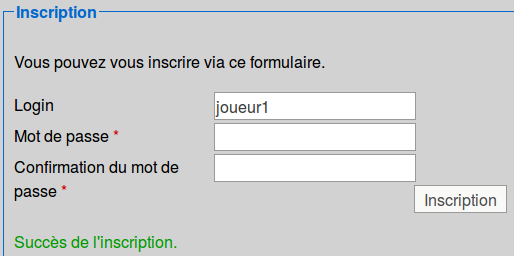
\includegraphics[scale=0.36]{../graph/2.1-inscriptionsucces.png} 
      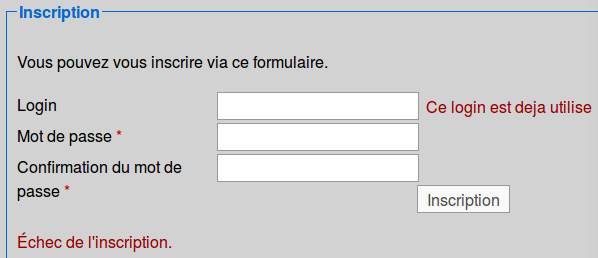
\includegraphics[scale=0.36]{../graph/2.2-inscriptionechec.png} 
    \end{figure}

    \subsubsection{Connexion}
    Maintenant que le joueur est inscrit, il peut se connecter via un autre formulaire où il lui ai demandé de saisir login et mot de passe (qui doivent toujours être valides). 
    \begin{figure}[H]
      \center
      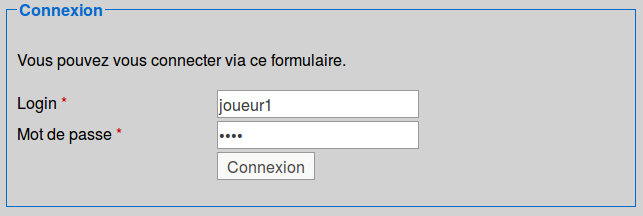
\includegraphics[scale=0.5]{../graph/3-connexion.png}
    \end{figure}

  \subsection{Joueur connecté}  
  Après avoir validé son formulaire de connexion, et si les identifiants ont bien été saisis, le joueur arrive sur une nouvelle page d'accueil dans laquelle on visulalise un menu horizontal ainsi que deux boutons : l'un permettant d'aller vers son \textbf{portefeuille}, et l'autre vers la \textbf{bourse}.
  \begin{figure}[H]
    \center
    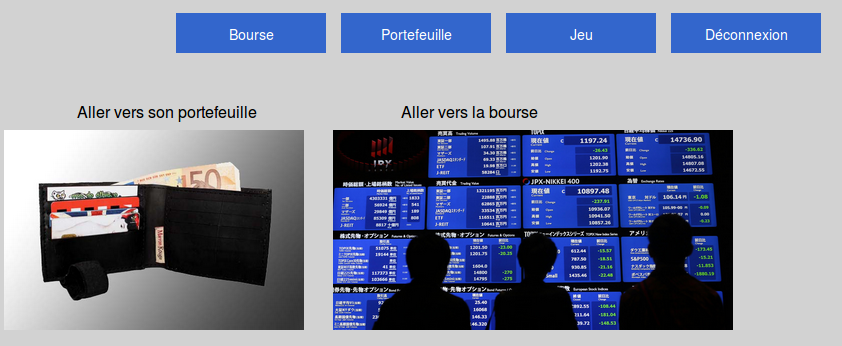
\includegraphics[scale=0.5]{../graph/4-accueilconnecte.png}
  \end{figure}
    
    \subsubsection{Bourse}
    Prenons le cas où il décide de consulter la \textbf{bourse}, ou plutôt l'échantillon de la bourse que le broker propose à ses clients. Dans un premier temps, le joueur arrive sur la page suivante (vide et une simple barre de recherche) : 
    \begin{figure}[H]
      \center
      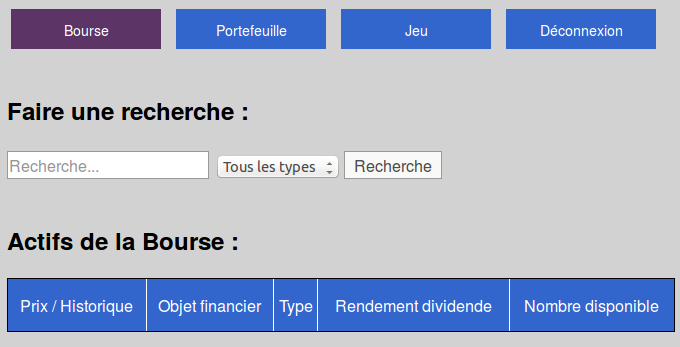
\includegraphics[scale=0.4]{../graph/5-accueilbourse.png}  
    \end{figure}
      
      \begin{enumerate}
       \item \textbf{Recherche :} le joueur peut effectuer une recherche par mot clés et/ou par type d'actif financier. Par exemple, l'utilisateur peut saisir 'app' et choisir 'Action' en espérant obtenir l'action de la société Apple (si elle existe dans l'échantillon). La recherche s'effectue et on voit s'afficher toutes les \textbf{actions} ayant les lettres 'aap' (peu importe la casse) dans le libellé ou dans le code. On voit alors le résultat de la recherche qui se compose de 3 actions avec le détail de celles-ci. 
      \begin{figure}[H]
	\center
	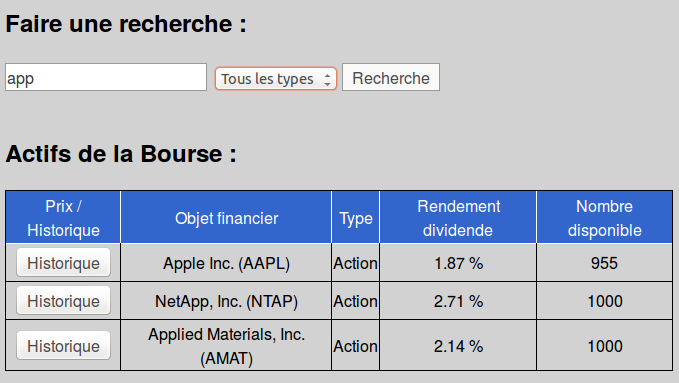
\includegraphics[scale=0.5]{../graph/5-rechercheactifs.png}
      \end{figure}
      
      La même chose peut s'effectuer sur une recherche sans mot clé et seulement sur les obligations :\\
      \begin{figure}[H]
	\center      
	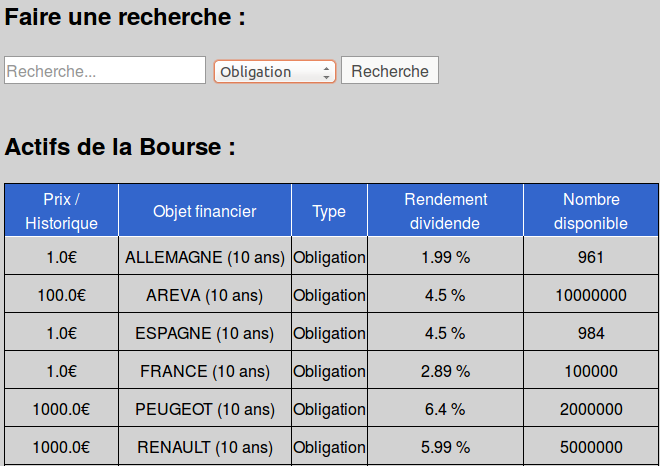
\includegraphics[scale=0.5]{../graph/5-rechercheobligations.png}
      \end{figure}
      
      On suppose finalement que la recherche abouti au résultat suivant et que le joueur souhaite en savoir plus sur cette action et clique sur le bouton \textbf{Historique}.\\	
      \begin{figure}[H]
	\center      
	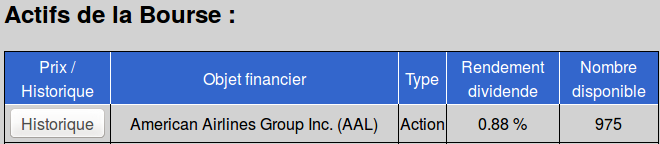
\includegraphics[scale=0.5]{../graph/5-detailaction.png}
      \end{figure}
      
      \item \textbf{Historique :}
      \begin{figure}[H]
	\center
	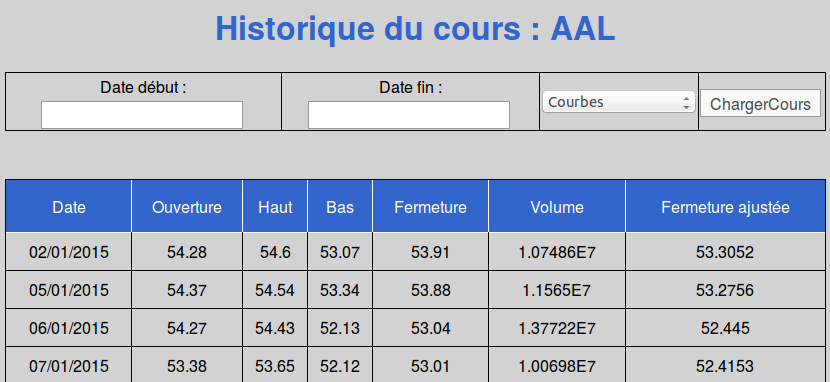
\includegraphics[scale=0.5]{../graph/6-historiquetableau.png}
      \end{figure}
      \begin{figure}[H]
	\center
	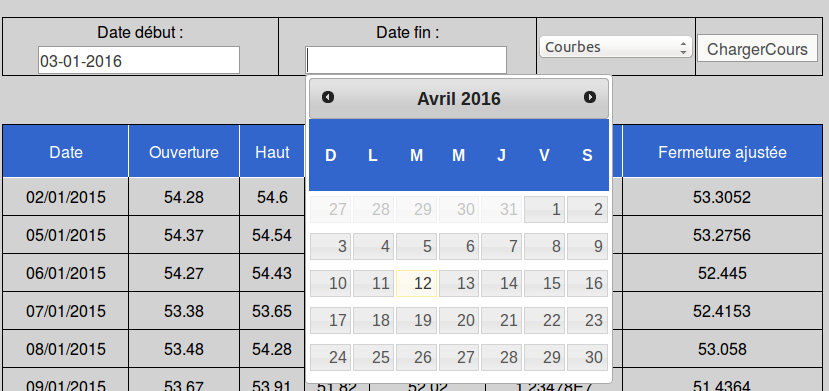
\includegraphics[scale=0.5]{../graph/6-recherchecalendrier.png}
      \end{figure}
      \begin{figure}[H]
	\center
	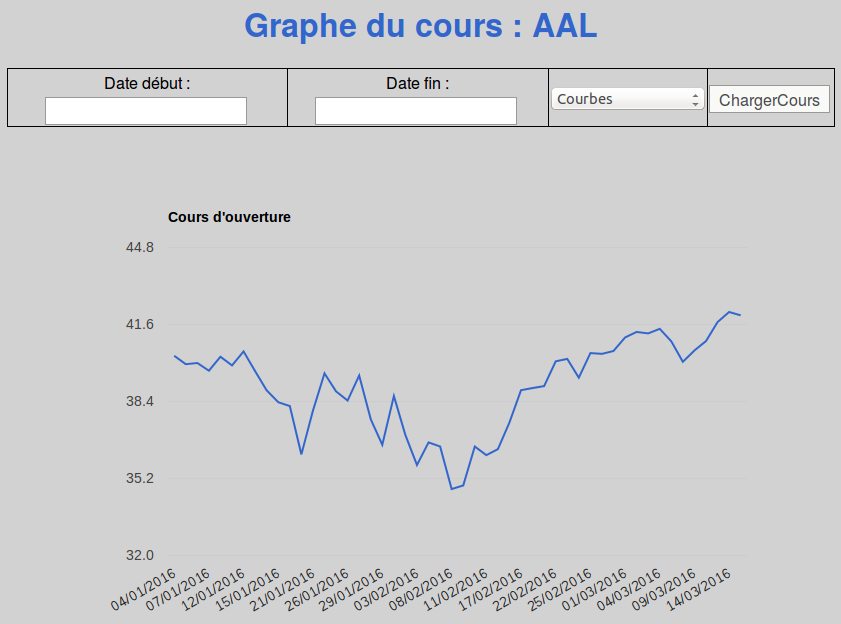
\includegraphics[scale=0.5]{../graph/6-historiquecourbe.png}
      \end{figure}
      \begin{figure}[H]
	\center
	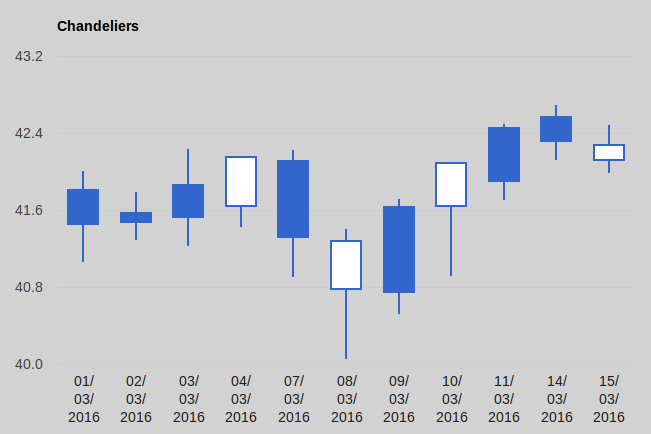
\includegraphics[scale=0.5]{../graph/6-historiquechandeliers.png}
      \end{figure}
      \begin{figure}[H]
	\center
	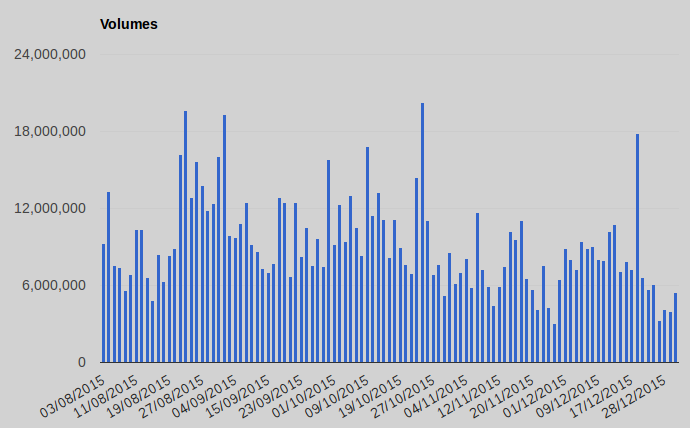
\includegraphics[scale=0.5]{../graph/6-historiquevolumes.png}
      \end{figure}
      \begin{figure}[H]
	\center
	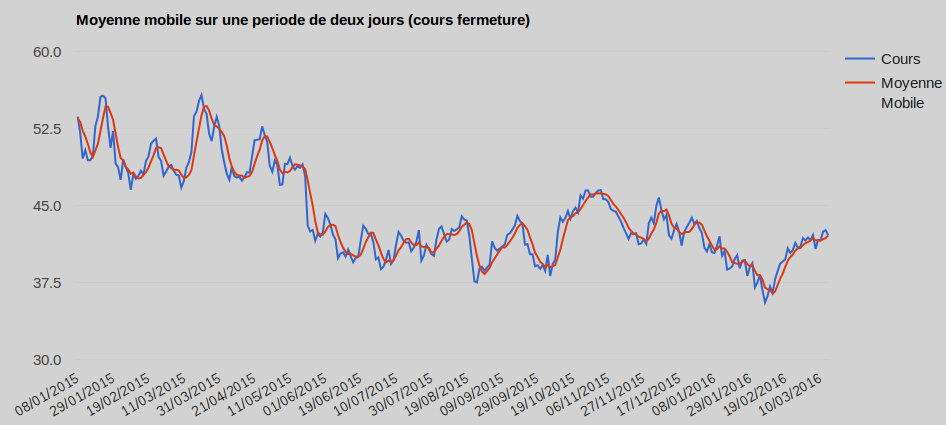
\includegraphics[scale=0.5]{../graph/6-historiqueMoyMob.png}
      \end{figure}
      \begin{figure}[H]
	\center
	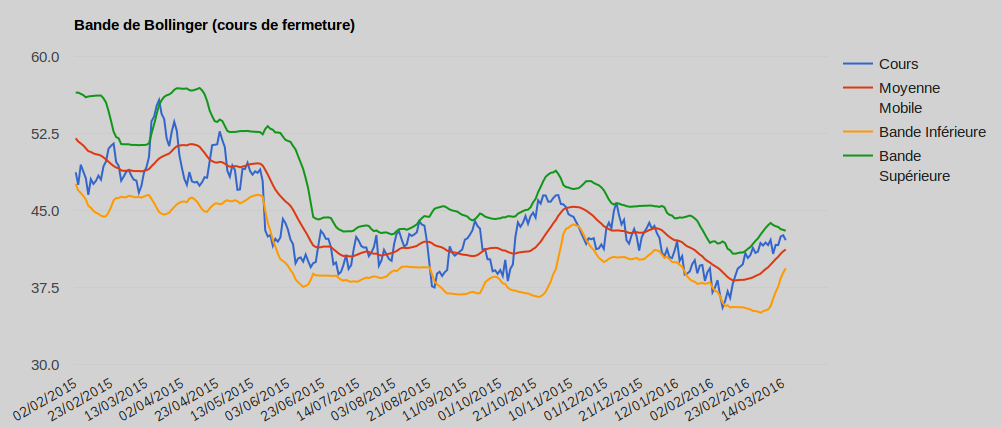
\includegraphics[scale=0.5]{../graph/6-historiqueBollinger.png} 
      \end{figure}
      
      \end{enumerate}
    
    \subsubsection{Portefeuille}
    \begin{figure}[H]
      \center
      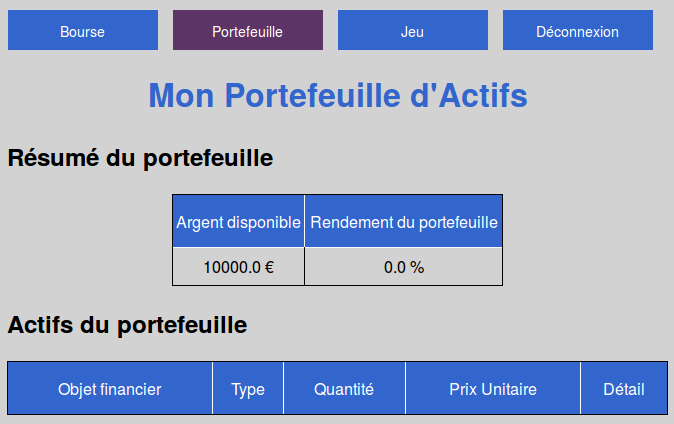
\includegraphics[scale=0.5]{../graph/7-accueilportefeuillevide.png}
    \end{figure}
      
      Achat d'actifs financiers
      \begin{figure}[H]
	\center
	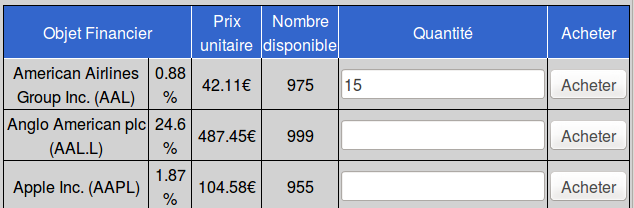
\includegraphics[scale=0.5]{../graph/7-achataction.png}
	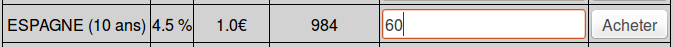
\includegraphics[scale=0.5]{../graph/7-achatobligation.png}
	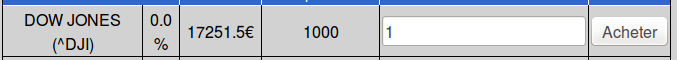
\includegraphics[scale=0.5]{../graph/7-achatindicetropcher.png}
	
\includegraphics[scale=0.5]{../graph/7-achatindiceechec.png}
	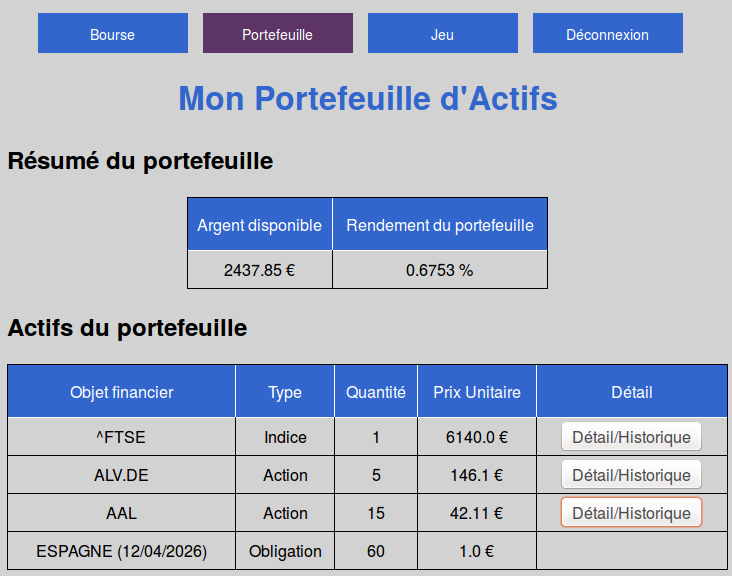
\includegraphics[scale=0.5]{../graph/7-vueportefeuilleapresachats.png}
      \end{figure}
      
      Vente d'actifs financiers
      \begin{figure}[H]
	\center
	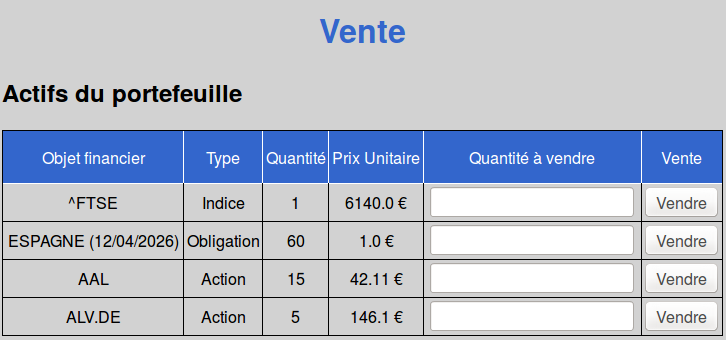
\includegraphics[scale=0.5]{../graph/7-vente.png}
	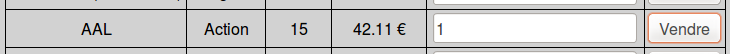
\includegraphics[scale=0.5]{../graph/7-vente1action.png}
	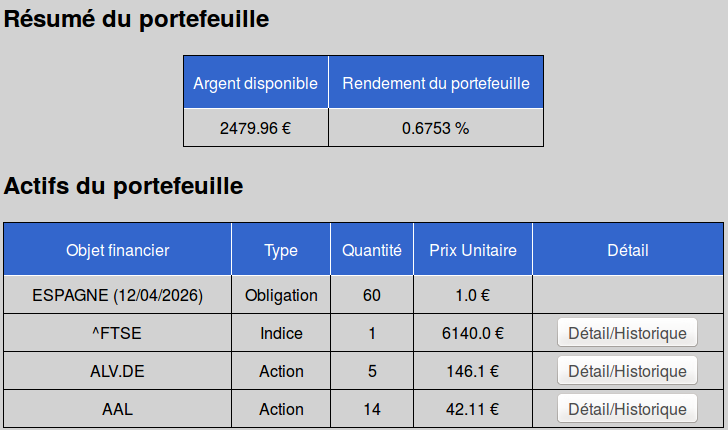
\includegraphics[scale=0.5]{../graph/7-accueilapresvente.png}
      \end{figure}
	
      Indicateurs
      \begin{figure}[H]
	\center
	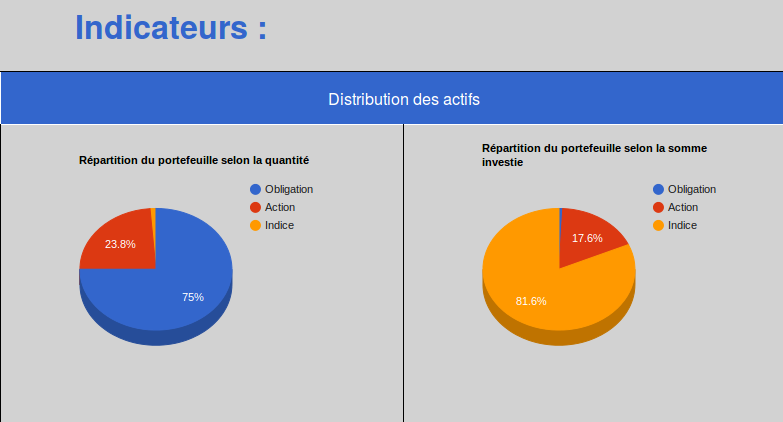
\includegraphics[scale=0.5]{../graph/7-indicateursPtfcamemberts.png}
	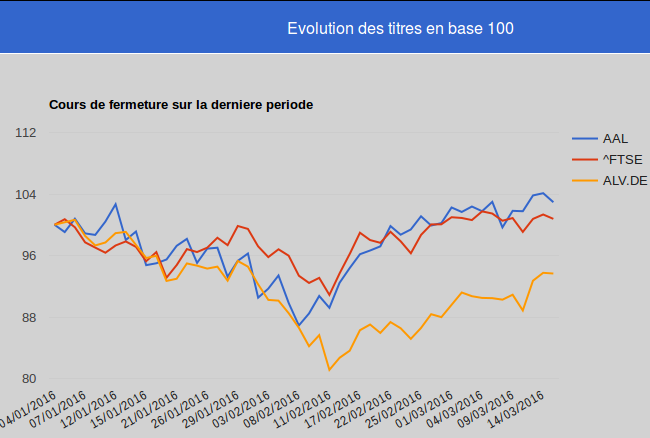
\includegraphics[scale=0.5]{../graph/7-indicateursbase100.png}
      \end{figure}

      Exporter  
      \begin{figure}[H]
	\center	
	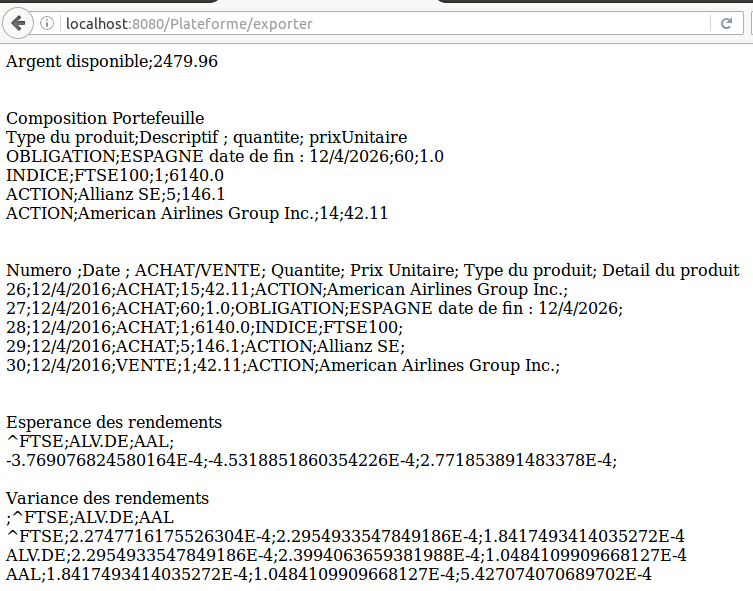
\includegraphics[scale=0.5]{../graph/7-exporterpage.png}
      \end{figure} 
  
    \subsubsection{Jeu}
    \begin{figure}[H]
      \center
      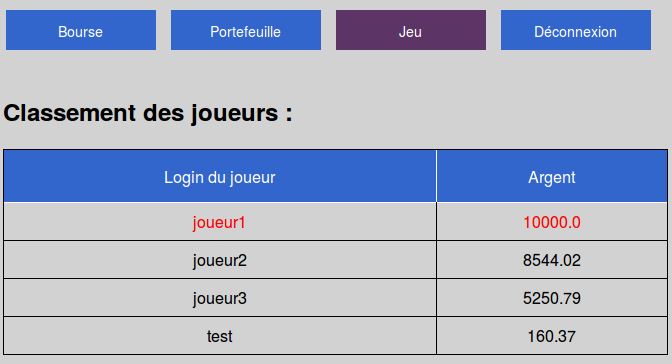
\includegraphics[scale=0.5]{../graph/8-jeuclassement.png}
      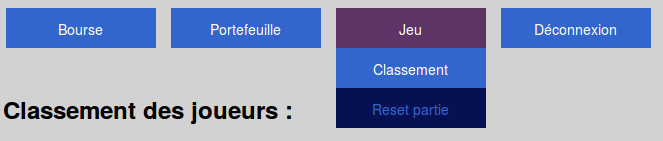
\includegraphics[scale=0.5]{../graph/8-jeuresetpartie.png}
    \end{figure} 

    Déconnexion